% Si tu trabajo incluye anexos, puedes descomentar las siguientes líneas
\chapter* {Annex}
\label{chap:annexes}
\pagenumbering{gobble} % Las páginas de los anexos no se numeran



\section{Optimization results for all the models}

The results are shown in a graphical way, as the tables (originally stored in an Excel spreadsheet) contain conditional formatting, showing the inference speed in a color scale.

\subsection{Object detection models}

\begin{figure}[h]
	\centering
	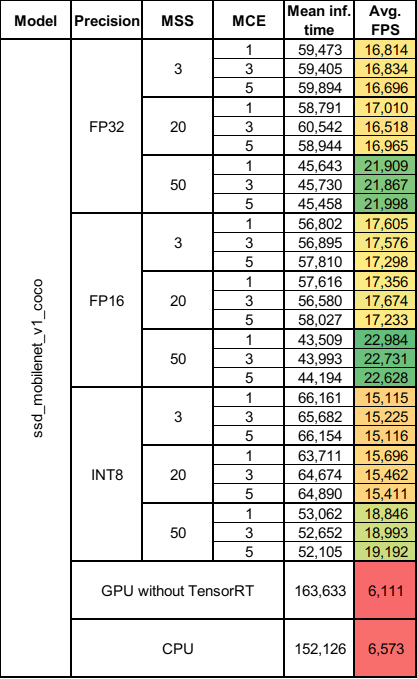
\includegraphics[width=0.5\linewidth]{optimizations_ssd_mobilenet_v1_coco}
	\caption{Optimization results for the object detection model \texttt{ssd\_mobilenet\_v1\_coco}.}
\end{figure}

\begin{figure}[h]
	\centering
	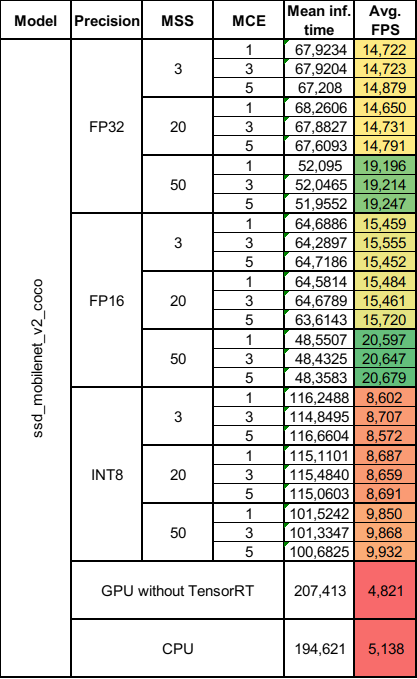
\includegraphics[width=0.5\linewidth]{optimizations_ssd_mobilenet_v2_coco}
	\caption{Optimization results for the object detection model \texttt{ssd\_mobilenet\_v2\_coco}.}
\end{figure}

\begin{figure}[h]
	\centering
	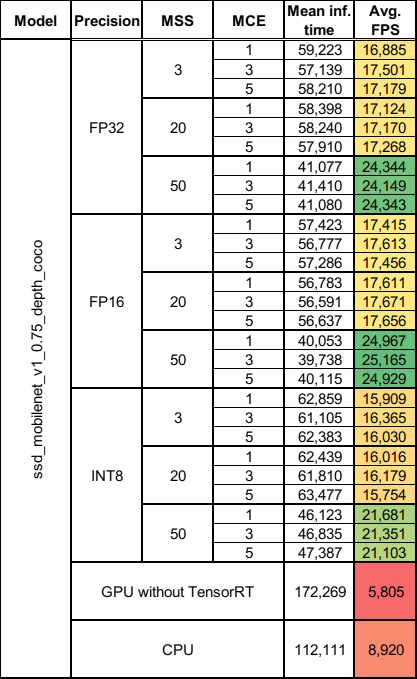
\includegraphics[width=0.5\linewidth]{optimizations_ssd_mobilenet_v1_0.75_depth_coco}
	\caption{Optimization results for the object detection model \texttt{ssd\_mobilenet\_v1\_0\.75\_depth\_coco}.}
\end{figure}

\begin{figure}[h]
	\centering
	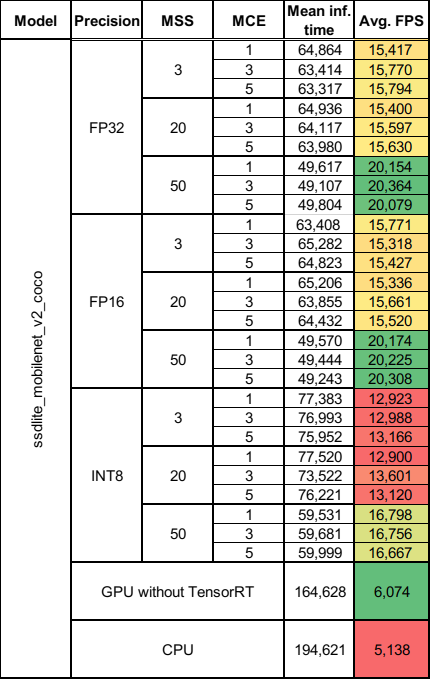
\includegraphics[width=0.5\linewidth]{optimizations_ssdlite_mobilenet_v2_coco}
	\caption{Optimization results for the object detection model \texttt{ssdlite\_mobilenet\_v2\_coco}.}
\end{figure}

\begin{figure}[h]
	\centering
	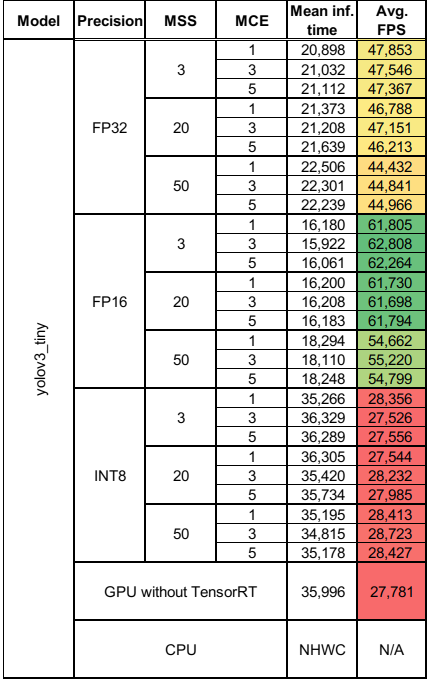
\includegraphics[width=0.5\linewidth]{optimizations_yolov3_tiny}
	\caption{Optimization results for the object detection model \texttt{yolov3\_tiny} (due to hardware compatibility issues, the CPU testing was impossible to perform).}
\end{figure}

\subsection{Face detection models}

These models are the specifically trained for the \texttt{faced} library \cite{faced}. They have been optimized as well, swapping the originally included models in the package for the TensorRT optimized ones.

\begin{figure}[h]
	\centering
	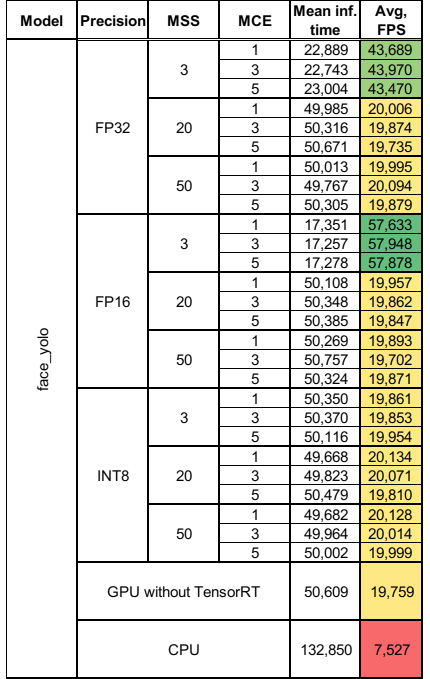
\includegraphics[width=0.5\linewidth]{optimizations_face_yolo}
	\caption{Optimization results for the face detector model \texttt{face\_yolo}.}
\end{figure}

\begin{figure}[h]
	\centering
	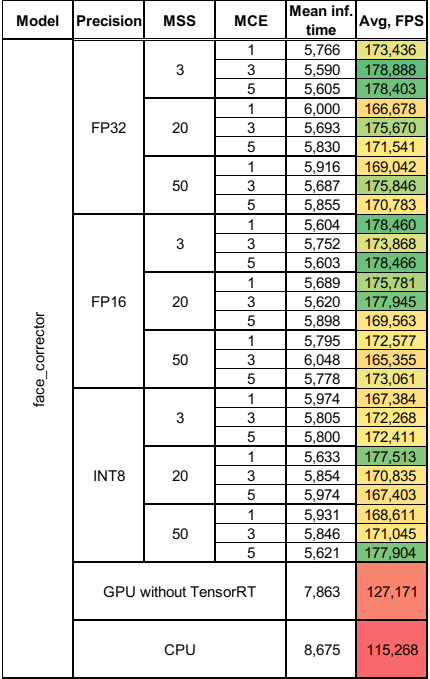
\includegraphics[width=0.5\linewidth]{optimizations_face_corrector}
	\caption{Optimization results for the face corrector mdoel \texttt{face\_corrector}.}
\end{figure}


\subsection{Face encoding model}
This is the FaceNet implementation \cite{facenet}, which has been optimized as well using TensorRT:

\begin{figure}[h]
	\centering
	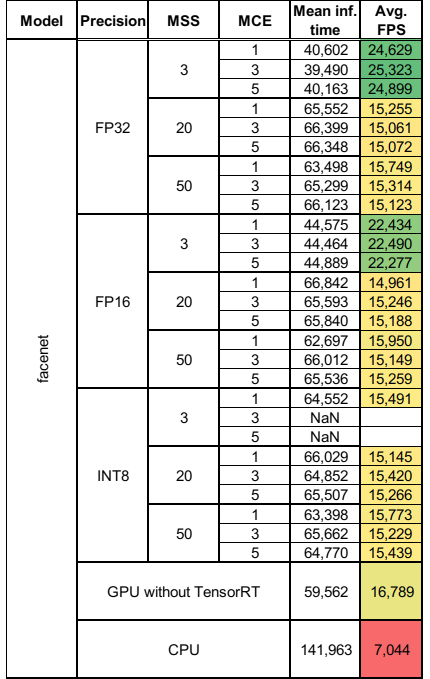
\includegraphics[width=0.5\linewidth]{optimizations_facenet}
	\caption{Optimization results for the face encoding model \texttt{facenet}.}
\end{figure}